44444444444
\chapter{引言}
\label{chap:gioi_thieu}

\section{研究背景与选题理由}
\label{sec:boi_canh_ly_do}

\subsection{全球背景:质量保障成为必然趋势}

进入21世纪,高等教育(GDĐH)已超越其作为知识保存与传播场所的传统角色,成为决定各国竞争力和可持续发展的战略驱动力\footcite{Altbach2001}\footcite{WB_KnowledgeEconomy}。在基于知识的全球化经济(knowledge-based economy)背景下,大学被视为“创新引擎”,是培养高素质人力资源、产出科学技术发明以及为社会复杂挑战提供解决方案的场所\footcite{OECD_HE2008}。这一角色的转变对高等教育体系的质量提出了前所未有的紧迫要求。质量不再是学术象牙塔中的抽象概念,而已成为一个可衡量、可比较的因素,是国际舞台上激烈竞争的标准。

正是在这样的背景下,质量保障体系(ĐBCL - Quality Assurance),特别是外部质量保障(External Quality Assurance - EQA),已成为不可逆转的全球趋势。根据世界银行(World Bank)和联合国教科文组织(UNESCO)的报告,在过去几十年里,建立国家级质量保障机构的国家数量急剧增加,覆盖了全球几乎所有地区\footcite{WorldBank_QA_GlobalTrends}\footcite{UNESCO_QA2018}。这一强劲的扩散势头主要由三大动力推动:

\begin{enumerate}
    \item \textbf{高等教育的大众化 (Massification of Higher Education):} 学生规模和大学数量的爆炸性增长,包括私立院校的迅猛发展,使得高等教育体系变得前所未有的多样化和复杂化。这种多样性虽然带来了更多的教育机会,但同时也带来了质量下降和不均衡的风险。因此,政府和社会需要一个外部监督机制,以确保整个体系的最低质量门槛\footcite{Trow2007}。
    
    \item \textbf{问责制要求的提高 (Increased Demand for Accountability):} 随着公共财政和学习者对高等教育投入的日益增加,对大学问责制的要求也越来越高。包括政府、家长、学生和雇主在内的各利益相关方都想知道他们的投资是否带来了应有的效益。外部质量保障体系及其认证活动和结果公开,是履行这一问责制的最重要工具\footcite{Harvey2005}。
    
    \item \textbf{跨境教育的兴起 (Rise of Cross-border Education):} 全球化极大地促进了学生、教师和教育项目跨越国界的流动。这产生了对学位和学分互认的迫切需求。一个可靠的、其标准与国际惯例接轨的质量保障体系,是一个国家参与全球教育市场、吸引国际学生并确保本国学生文凭在国外获得承认的先决条件\footcite{Knight2006}。
\end{enumerate}

这些动力已将质量保障从一项纯粹的专业活动转变为一项重要的国家治理工具,是现代高等教育体系结构中不可或缺的要素。清晰理解这些全球趋势和动力,是准确分析像越南这样的特定国家质量保障体系所面临的背景与挑战的第一步。

\subsection{区域背景:东盟共同体内的质量协调化}
\label{subsec:boi_canh_khu_vuc}

如果说全球背景带来了竞争与融合的压力,那么区域背景则提出了合作与协调的要求。对越南而言,最重要的区域背景是东盟共同体。2015年东盟经济共同体(AEC)的成立设定了一个宏伟目标:建立一个统一的市场和生产基地,允许商品、服务、投资、资本以及特别是技术劳工(skilled labor)的自由流动\footcite{ASEAN_AEC_Blueprint}。

为实现这一目标,教育水平与质量的协调化及互认成为一项核心要求。在河内接受培训的工程师,需要具备与在曼谷或吉隆坡的雇主所承认的同等能力和文凭。深刻认识到这一要求,区域内的教育领导者们已率先努力建设一个共同的高等教育空间。实现这一努力最重要的工具是东盟大学网络(ASEAN University Network - AUN),特别是其下属的质量保障网络——AUN-QA(ASEAN University Network - Quality Assurance),该网络成立于1998年\footcite{AUNQA_History}。

AUN-QA并非一个具有强制权力的超国家认证机构,而是一个基于自愿、合作和同行学习(peer learning)原则运作的网络。其使命如官方文件所述,是“推动东盟高等教育机构的质量保障,提升高等教育质量,并为东盟共同体的共同利益与区域及国际机构合作”\footcite{AUN-QAGuide}。

AUN-QA的运作理念可概括为\textbf{“多元中的和谐”}原则。该网络不寻求消除各国教育体系之间的差异,而是建立一套共同的标准和评估流程,作为质量的“公分母”和通用语言。AUN-QA标准(目前是针对课程层级的4.0版)包含8项标准和明确的子标准,已成为该地区大学的重要参考框架。同行评审(peer review)流程,即由成员大学的专家相互评估,不仅有助于确保客观性,还创造了一个极其有效的经验和最佳实践分享机制\footcite{AUNQA_Report2023}。

对越南而言,积极参与AUN-QA网络具有战略意义。这不仅是提升国内大学质量和声誉的渠道,也是融入区域高等教育空间最快、最有效的途径。一个教育项目获得AUN-QA认证是其质量的重要保证,有助于该项目的毕业生在东盟劳动力市场上获得更多优势。因此,任何关于越南质量保障体系的分析都不能忽视AUN-QA框架作为区域背景重要因素的角色和影响。


\subsection{2015-2024年阶段越南高等教育发展背景:现状分析}

2015-2024年阶段标志着越南高等教育体系的一个重要转型时期。该体系已从注重扩大规模以满足社会学习需求,逐渐转向优先提升质量、调整结构和国际融合。分析此阶段的官方统计数据,将提供一幅全景图,突显越南高等教育所取得的成就、发展趋势以及面临的挑战,从而明确一个有效的外部质量保障体系产生的背景及其紧迫性。

\subsubsection{系统规模与结构的发展}

过去十年,越南高等教育最显著的特点之一是培养规模的急剧增长,而教育机构数量则在有控制地增长,体现了国家的战略导向。

\paragraph{关于教育机构数量:}
大学体系实现了稳定和可持续的发展。2015年,全国共有214所高等教育机构\footcite{stat_quy_mo_2015_2021},到2024年,这一数字增至\textbf{243所},其中包括176所公立大学和67所私立大学\footcite{stat_moet_2024}。近十年间仅净增约29所学校,表明政策不鼓励大规模新建学校,而是侧重于巩固和提升现有机构的质量。这为在整个体系内进行管理和质量保障工作创造了更有利的环境。

\paragraph{关于学生规模:}
与学校数量的稳定增长相反,学生规模实现了飞跃。大学生总规模从2015年的\textbf{175.3万}人猛增至2024年的\textbf{235.6万}人\footcite{stat_moet_2024}\footcite{stat_quy_mo_2015_2021}。这表明社会对大学学习的需求日益增长,高等教育体系已努力满足这一需求。

\begin{figure}
    \centering
    % Placeholder for the chart. Replace with your actual chart image.
    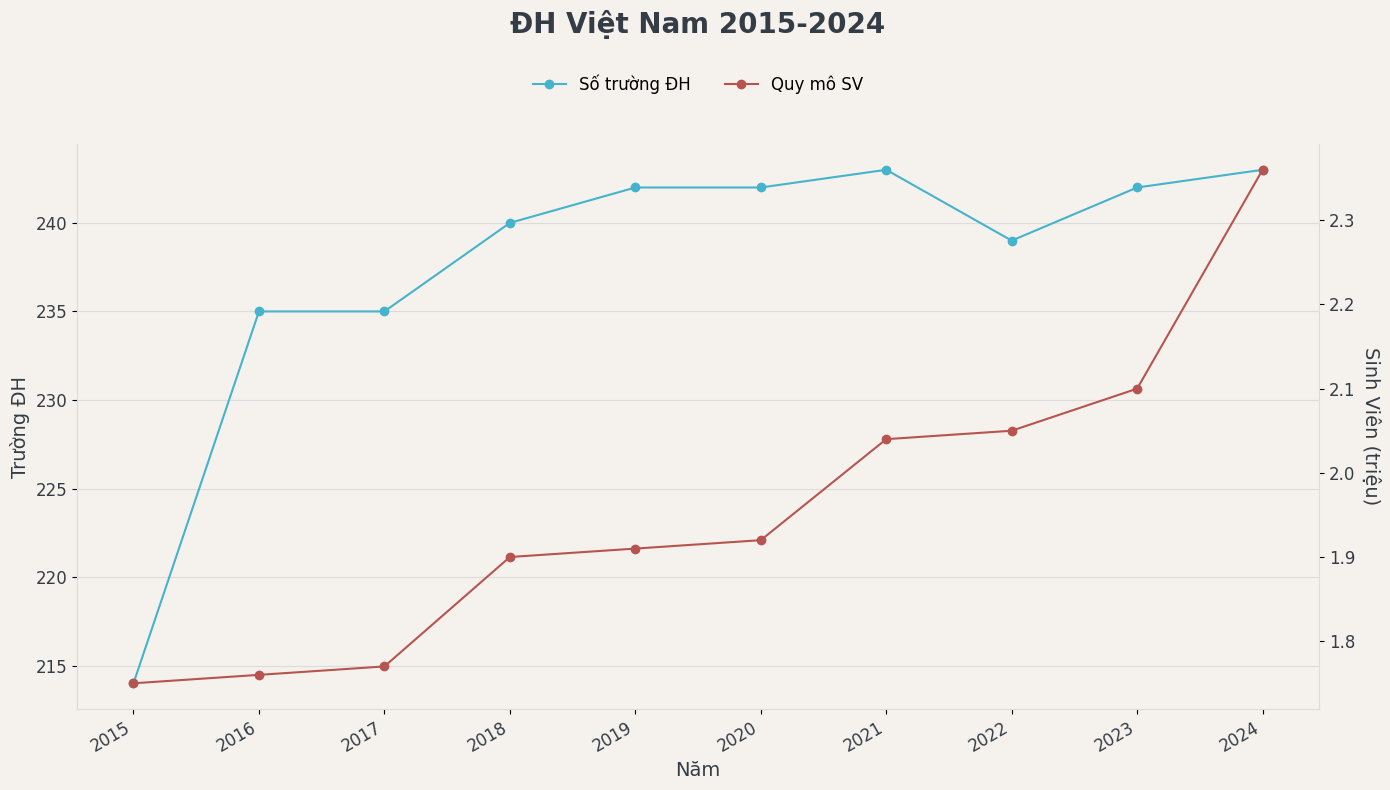
\includegraphics[width=0.9\textwidth]{image/bieu do 1 luan giao duc.png} 
    \caption{越南大学生规模与高校数量增长情况(2015-2024年)}
    \label{fig:quy_mo_phat_trien}
    \vspace{0.2cm}
    \footnotesize{\textit{来源:综合整理自越南教育培训部的数据\footcite{stat_moet_2024}及相关报告\footcite{stat_quy_mo_2015_2021}。}}
\end{figure}

特别是,2023-2024学年实现了突破性增长,比上一学年增加了\textbf{319,022}名学生\footcite{stat_moet_2024}。这并非寻常的线性增长,而是一次规模上的\textbf{飞跃(leap)},如图(图\ref{fig:quy_mo_phat_trien})所示。这种突增并非偶然现象,可以解释为多种政策和社会因素同时汇聚的结果,为整个体系带来了“推力”。

\paragraph{潜在原因分析:}
最直接和最重要的原因之一可能是各大学\textbf{招生政策的变化和招生指标的增加}。这一时期,除了传统的基于高中毕业考试成绩的录取方式外,多样化的录取方式也得到了大力发展。各大学加强使用学业成绩审查、自主能力评估考试等方式,为考生开辟了更多的“大门”。当大学,特别是民办大学和自主办学的公立大学,在确定招生指标和录取方式方面被赋予更多自主权时,它们倾向于扩大规模以满足社会需求和优化资源。整个体系招生指标的增加,结合灵活的录取方式,为前所未有的大量考生被录取和入学创造了条件。

第二个原因来自\textbf{经济社会因素和观念的转变}。COVID-19疫情后时期(2020-2022年)对劳动力市场和职业选择产生了一定影响。可能有一大部分学生和家庭意识到,对于没有高等专业水平的人来说,劳动力市场存在不确定性,从而坚定了大学文凭是未来稳定生活的必要“保险单”的信念。社会观念中“普及大学教育”的压力,推动了更大部分高中毕业生决定追求更高层次的学术道路,而不是进入劳动力市场或其他职业教育体系。

最后,这种突增是\textbf{共振效应}的结果。越南教育培训部扩大招生自主权的政策,如同一个“泄压阀”,释放了社会长期以来积累的“需求压力”。当大学之门比以往任何时候都更加敞开时,大量的社会学习愿望在同一个学年得以实现,从而造成了规模上的飞跃。

然而,规模的快速增长也正是对质量保障工作的最大挑战。它提出了一个紧迫的问题:师资队伍、物质设施,特别是内部质量管理流程的发展,是否能跟上学生数量的增长速度?这正是现实背景,要求一个外部质量保障体系必须有效运作,既能监督,又能支持各大学克服这一挑战。

\paragraph{关于学生结构与民办院校的角色:}
民办大学的发展是教育社会化的一个亮点。就读于民办学校的学生比例已逐渐增加,从2015年的约20\%上升到2024年的\textbf{22.76\%},学生人数达到536,295人\footcite{stat_moet_2024}。这一数字不仅显示了私营部门日益重要的贡献,也表明越南已**提前实现了政府第35号决议中提出的到2025年民办学生比例达到22.5\%的目标**。民办院校的壮大创造了一个良性竞争的环境,推动公立学校不断创新和提高质量。

\subsubsection{招生工作现状与专业选择趋势分析}

分析招生数据不仅能展现体系的输入端情况,还能反映年轻一代的职业选择趋势,这是质量保障体系需要掌握并作出相应调整的重要因素。

\paragraph{参与比例与招生结果:}
近年来,参加高中毕业考试的考生数量一直稳定在100万以上\footcite{stat_tuyen_sinh_2024_so_lieu}\footcite{stat_thi_sinh_2024}。值得注意的是,申请大学录取的考生比例占了很大一部分,2024年约占参考考生总数的\textbf{68.5\%},显示进入大学仍然是大多数学生的首选。

被录取后确认入学的考生比例是反映培养项目吸引力和契合度的重要指标。在2022年短暂下降(80.34\%)后,该比例已恢复并于2024年达到\textbf{81.87\%},共有551,497名考生确认入学\footcite{stat_nhap_hoc_2024}\footcite{stat_tuyen_sinh_2024_so_lieu}。

% --- CHÈN BIỂU ĐỒ 2 ---
% --- CHÈN BIỂU ĐỒ (PHIÊN BẢN ĐÃ CẬP NHẬT) ---
\begin{figure}[h!]
    \centering
    % Thay thế bằng tên file ảnh mới bạn vừa tạo bằng Python
    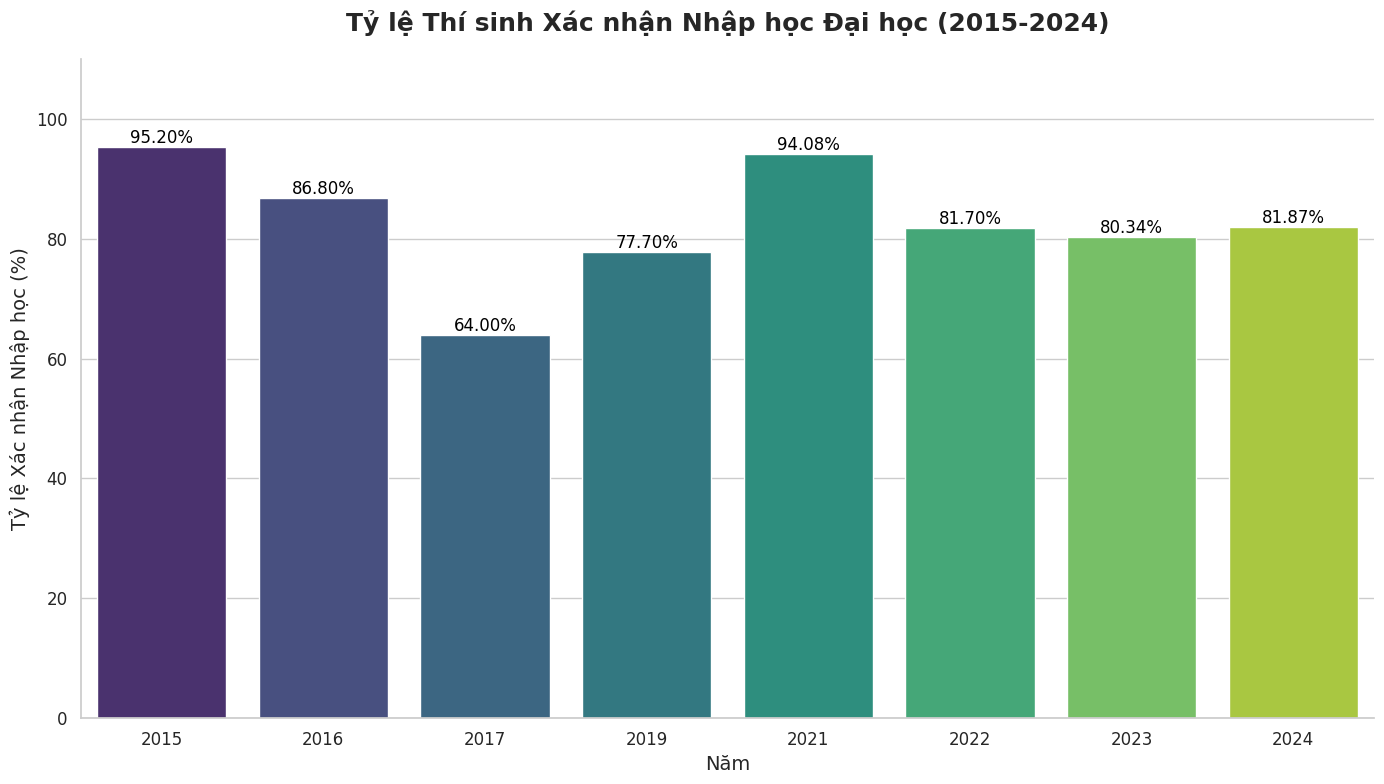
\includegraphics[width=0.8\textwidth]{image/ty_le_nhap_hoc_2015-2024.png}
    
    % Cập nhật caption cho đúng giai đoạn
    \caption{大学新生确认入学比例(2015-2024年)}
    \label{fig:ty_le_nhap_hoc_full}
    \vspace{0.2cm}
    
    % Cập nhật dòng nguồn với đầy đủ các trích dẫn
    \footnotesize{\textit{来源:综合整理自越南教育培训部及各新闻媒体历年数据 
    \footcite{ref1}\footcite{ref2}\footcite{ref3}\footcite{ref5}\footcite{ref7}\footcite{ref12}\footcite{ref19}\footcite{stat_nhap_hoc_2024}。}}
\end{figure}

这表明社会对高等教育体系的信心正在得到巩固。高入学率也意味着,平均每100名参加高中毕业考试的学生中,约有53人进入大学,这是过去9年来的最高比例,证实了越南已真正进入高等教育大众化阶段\footcite{stat_ty_le_vao_dh_2023}。

\paragraph{专业选择趋势:}
2024年的招生申请数据显示,专业选择趋势发生了显著变化。**教育科学与教师培养**类专业的志愿数量出人意料地大幅增长,比2023年增加了\textbf{85\%}。自然科学领域也吸引了大量关注,增幅达61\%\footcite{stat_tuyen_sinh_2024_so_lieu}。

相反,前些年的“热门”专业如**工商管理**(-3\%)和**计算机与信息技术**(-5\%)则出现了小幅下降趋势\footcite{stat_tuyen_sinh_2024_so_lieu}。这一转变可能反映了社会对长期人力资源需求的认知变化以及国家对教育行业的新政策。这是一个重要的信号,质量保障机构和各大学需要深入分析,以便及时调整培养结构。

\subsubsection{资源分析:师资队伍与物质设施}

一个教育体系的质量在很大程度上取决于其师资队伍的质量和保障条件。

\paragraph{关于师资队伍:}
2023-2024学年,全系统共有\textbf{88,031名全职教师}。在学历方面,有\textbf{28,862名教师拥有博士学位(占32.8\%)},49,229名教师拥有硕士学位(占55.9\%),其余为本科学历或其他学历\footcite{stat_moet_2024}。该学历结构如图\ref{fig:co_cau_giang_vien}所示。拥有博士学位的教师比例与前几年相比有了显著提高,这是提升培养和研究质量的重要前提。


% --- CHÈN BIỂU ĐỒ 3 ---
\begin{figure}[h!]
    \centering
    % Placeholder for the chart. Replace with your actual chart image.
    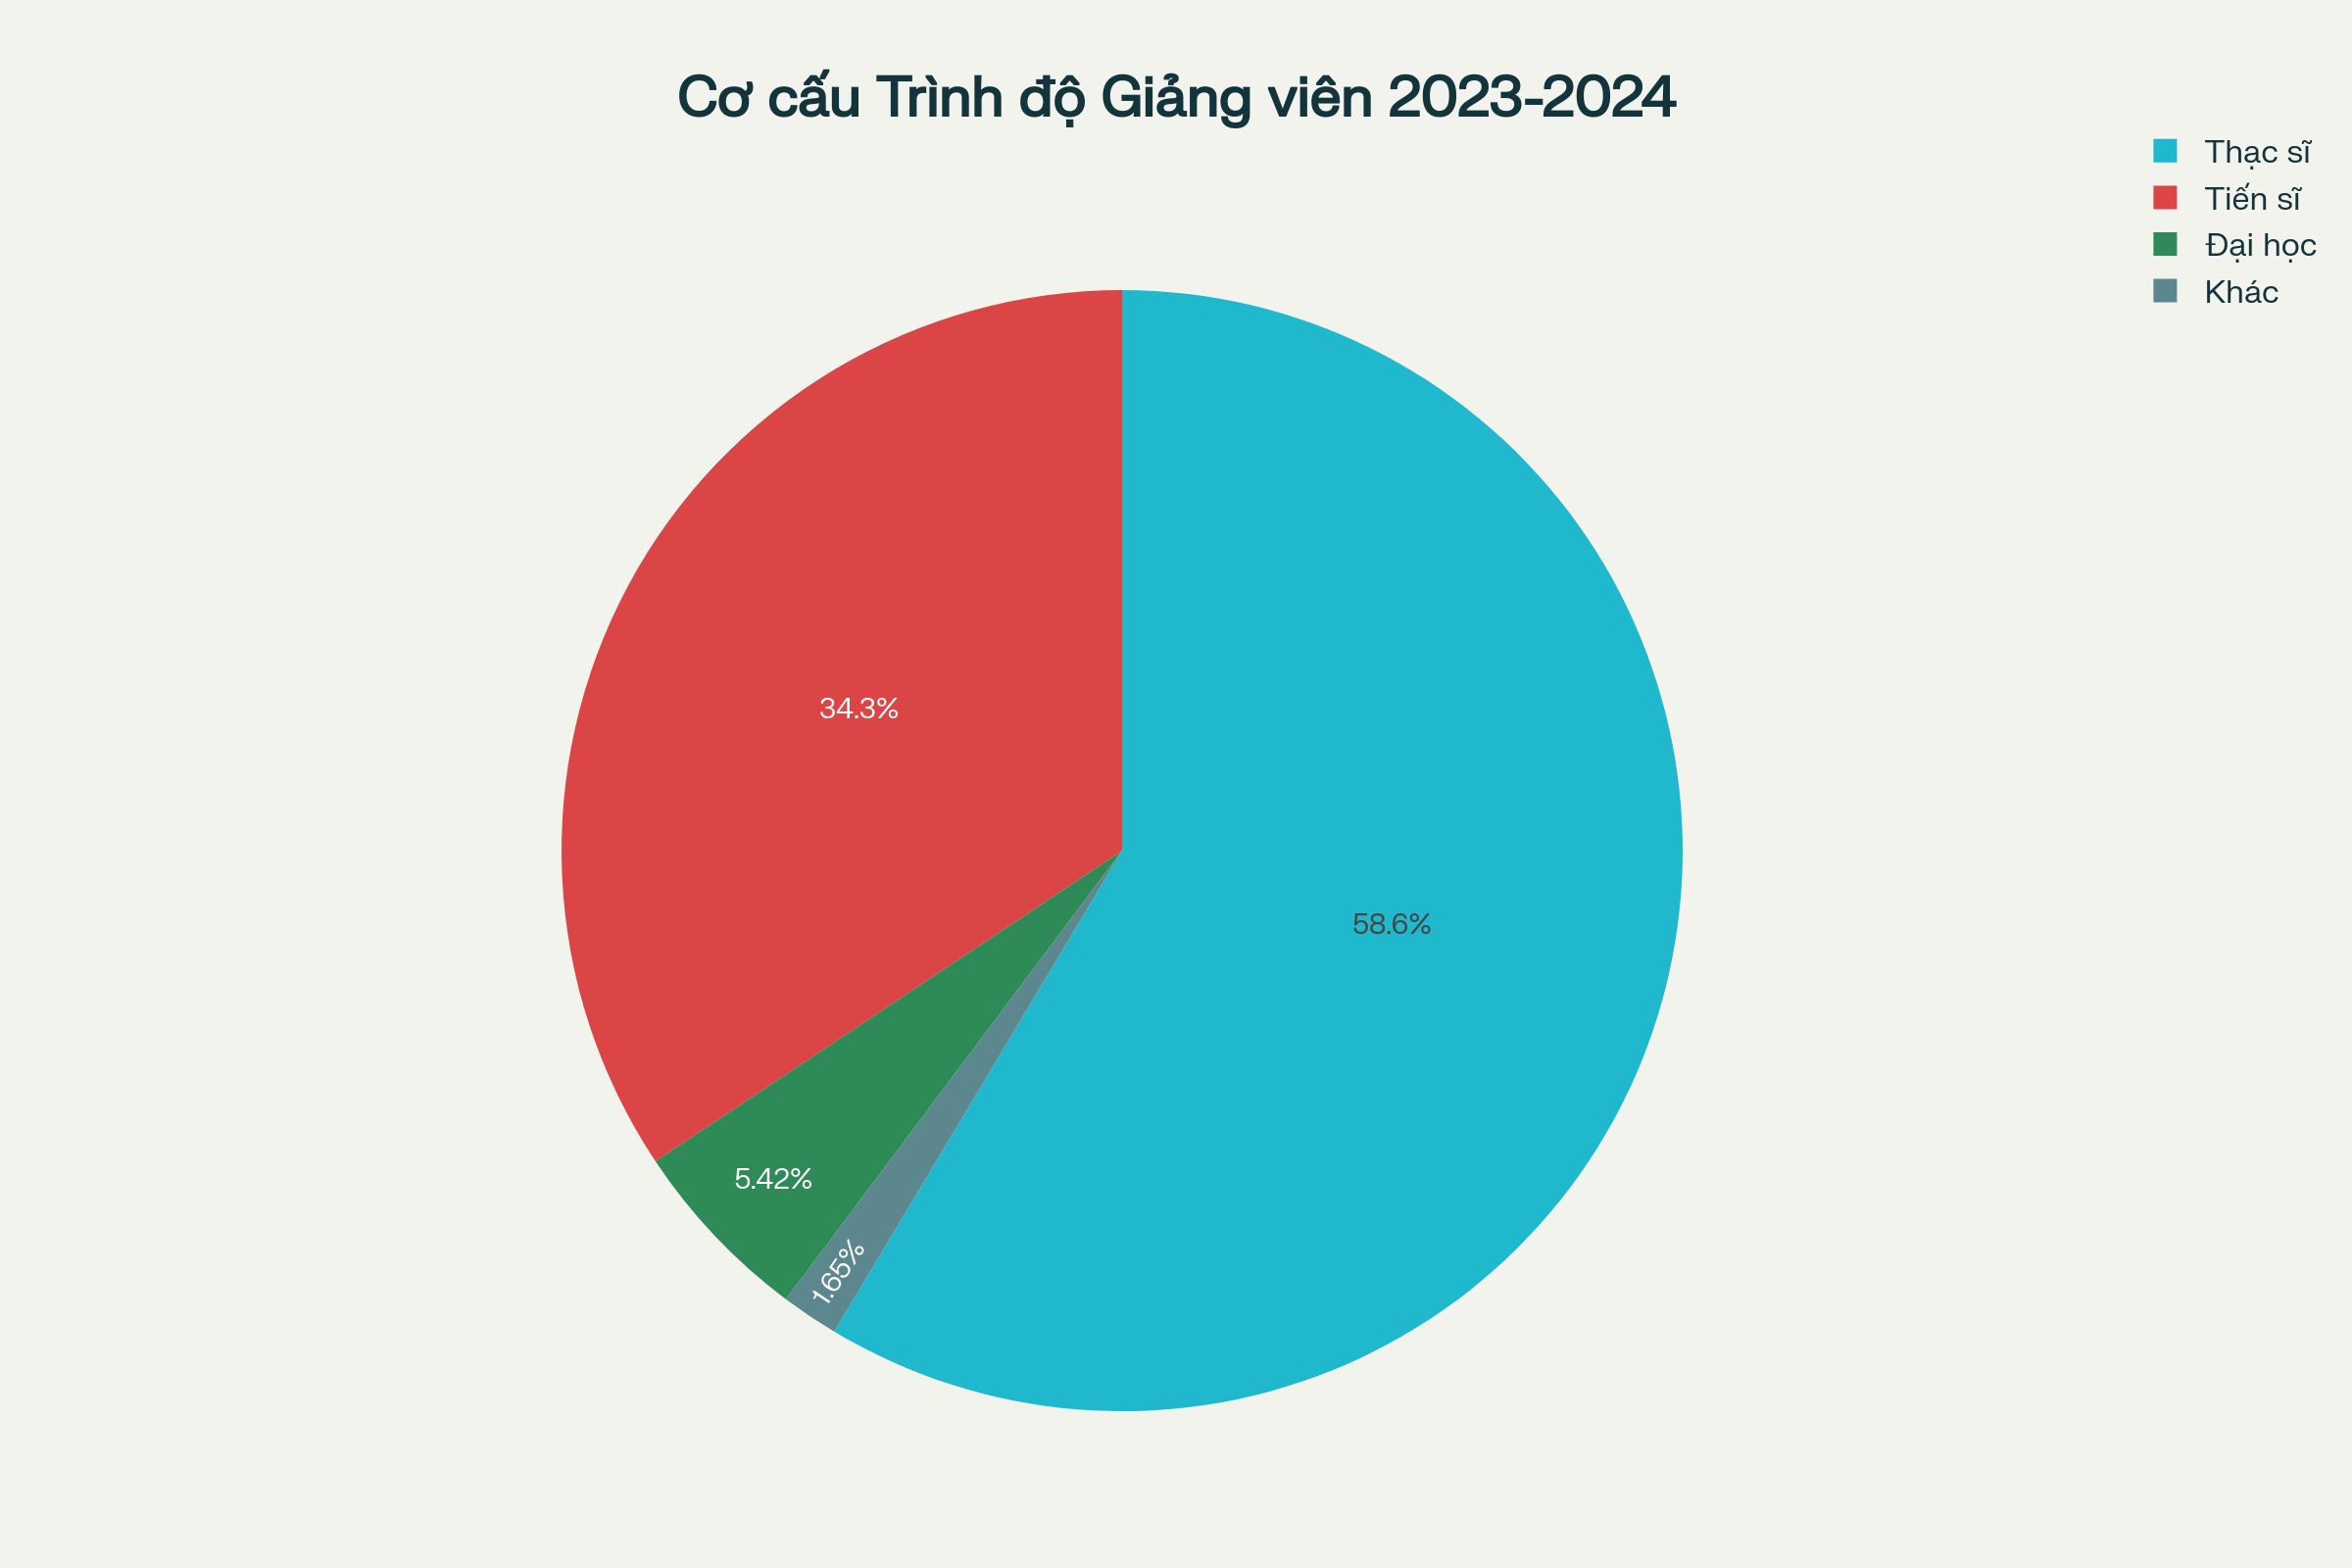
\includegraphics[width=0.6\textwidth]{image/co_cau_trinh_do_giang_vien_2023_2024.png}
    \caption{2023-2024学年全职教师学历结构}
    \label{fig:co_cau_giang_vien}
    \vspace{0.2cm}
    \footnotesize{\textit{来源:根据越南教育培训部数据计算\footcite{stat_moet_2024}。}}
\end{figure}

然而,生师比仍然偏高,尤其是在公立大学。全国平均生师比为公立大学30:1,民办大学22:1\footcite{stat_moet_2024}。公立大学的高生师比对确保师生之间有效互动(教育质量的核心要素)提出了巨大挑战。

\paragraph{关于资源分布:}
体系一个巨大且固有的挑战是地理分布上的严重不均衡。高质量的大学和师资队伍主要集中在红河三角洲(占学校总数的44.3\%)和东南部(18.4\%)两大重点经济区。而西原等贫困地区仅占学校总数的1.6\%\footcite{stat_quy_mo_2015_2021}\footcite{stat_phan_bo_dia_ly}。这种不平衡也明显体现在接受高等教育的机会上,红河三角洲的学生升入大学的比例(64.44\%)显著高于中北部山区(40.25\%)\footcite{stat_ty_le_vao_dh_2023}。这种差距要求质量保障政策必须考虑到地区因素,以确保公平和均衡发展。

\subsubsection{产出分析:毕业与就业}

产出质量是一个教育体系最终和最重要的衡量标准。
\begin{itemize}
    \item \textbf{毕业数量:} 2024年,高等教育体系为劳动力市场提供了\textbf{313,572名学士、工程师},与2023年的228,092人相比大幅增加\footcite{stat_moet_2024}。这表明高等教育在提供高水平人力资源方面扮演着越来越重要的角色。
    \item \textbf{就业情况:} 然而,这部分人力资源的质量仍然是一个问号。根据一份2018年的报告,毕业生毕业后就业率仅为\textbf{65.5\%}\footcite{stat_that_nghiep_2018}。更令人担忧的是,拥有大学、大专学历群体的失业率仍然高于中专学历群体。这表明所培养的技能与劳动力市场需求之间存在“不匹配”(mismatch),这是外部质量保障体系必须集中解决的核心问题。
\end{itemize}

\subsubsection{关于现状的初步结论}
对2015-2024年阶段统计数据的分析表明,越南高等教育正处于一个充满活力但又潜藏诸多挑战的发展阶段。
\begin{itemize}
    \item \textbf{成就:} 培养规模大幅扩展,满足了社会的学习需求;结构向民办领域积极转变;师资队伍的学历水平显著提高。
    \item \textbf{挑战:} 规模的急剧增长给质量带来了巨大压力;地区间资源分布不均的问题依然严峻;最重要的是,产出质量尚未能真正满足劳动力市场的要求。
\end{itemize}
这些挑战证实了建立一个强有力的外部质量保障体系的必要性,该体系不仅要监督合规性,还必须能够推动教育机构内部发生实质性变革,以解决质量和契合度的核心问题。


% done goi 2


\section{研究现状与研究问题综述}
\label{sec:tong_quan_nghien_cuu}

\subsection{研究背景与研究问题介绍}

如上文所分析,越南高等教育(GDĐH)的质量与质量保障问题及其挑战与机遇,近年来已引起众多学者、管理者和国际组织的关注。大量已发表的研究成果、政策报告和分析文章,为该领域构建了重要的知识基础。然而,一项新的研究要想做出真正的贡献,对现有成果进行系统化和批判性评估是不可或缺的一步。这一综述过程不仅旨在罗列已有的研究,更重要的是要识别那些“尚未探索的领域”、“悬而未决的问题”——换言之,即明确界定本论文旨在填补的\textbf{研究空白(research gap)}。

在此基础上,本论文确定其核心研究问题如下:

\begin{center}
\textit{一个在制度上不够强大、在适应变化背景方面不够灵活、在协调各相关方多样化要求方面不够全面的外部质量保障(ĐBCL)体系的缺失,正在对提升越南高等教育的实质性质量和国际竞争力的目标构成系统性障碍。}
\end{center}

为进一步阐明此问题,下文将从两大方面对相关研究进行综述:一是关于质量保障模型与理论的国际研究,二是以越南为具体背景的研究。

\subsection{关于质量保障模型与理论的国际研究综述}

世界范围内关于高等教育质量保障的研究经历了多个发展阶段,理论重心各不相同,为审视各国体系提供了丰富的视角。

在早期阶段,研究通常集中于描述认证机构的形成和结构,主要从公共管理和公共政策的角度出发。这些著作强调国家在制定规则和监督体系中的作用,这一方法接近于委托代理理论\footcite{Kivisto2008}\footcite{DeBoer2019}。其重点在于阐明国家与大学之间的问责关系。

进入一个更发展的阶段,组织社会学家开始应用新制度主义理论来解释为何质量保障模式在全球范围内呈现出扩散和趋同的趋势。Meyer、Powell、DiMaggio的著作已成为经典,他们指出大学的行为不仅基于技术效率,还受到寻求在制度环境中获得合法性的强大压力\footcite{MeyerPowell2020}\footcite{DiMaggioPowell1983}。后续如Kanwar等人(2019)的研究成功运用此理论框架,分析了在特定背景下推动应用质量保障的动力\footcite{Kanwar2019}。

近年来,随着质量保障体系变得日益复杂,研究者开始更多地关注不同主体之间的互动。利益相关者理论被越来越广泛地用于分析利益冲突以及将相关方(特别是学生和雇主)纳入质量保障流程的必要性。如Langrafe等人(2020)的研究提供了实证证据,表明利益相关者的参与与为学校和社会创造价值之间存在正相关关系\footcite{Langrafe2020}。

特别是,最新的研究已经认识到应用单一理论的局限性,并开始转向\textbf{综合与混合模型(hybrid models)}。欧洲大学协会(EUA)的报告经常强调从“控制”模式向“质量提升”模式的转变,其中外部评估流程旨在支持和促进内部的改进努力\footcite{EUA_Integration}\footcite{HarveyStensaker}。这种方法承认,一个有效的体系必须能够协调问责制和持续改进这两个目标。

\textit{从国际研究中得出的启示:}对国际文献的综述显示,关于质量保障的思维方式经历了明显的演变——从关注合规性控制,到解释制度压力,再到目前朝向综合、灵活和多方参与的模式发展。这表明,如果仅凭传统理论或仅描述政策规定来分析像越南这样的国家质量保障体系,将是不全面的。一个有深度的分析,需要将越南的体系置于这些理论和实践趋势的共同潮流中进行审视,同时识别其自身的独特性。



% done chuong 1 goi 3


\subsection{越南高等教育质量保障研究现状综述}
\label{subsec:tong_quan_vietnam}

在越南,高等教育质量与质量保障问题,已成为学术界和政策制定者高度关注的议题,尤其是在《高等教育法》颁布和修订之后。国内关于该领域的研究成果相当丰富,可分为三大类,每一类都有其独特的贡献与局限。

\paragraph{第一类:关于历史、政策与法律的研究。}
这是最普遍的研究类型,侧重于描述和系统化越南高等教育体系在各个时期的发展过程。黎文江(2003)等作者的著作,以及教育培训部各阶段的总结报告,为我们提供了从配给制时期到革新与融入时期的方针、政策变迁的全景视角\footcite{LeVanGiang2003}\footcite{MOET_50nam}。这些研究在史料方面价值很高,有助于理解现行质量保障政策的出台背景。然而,这类研究的主要局限在于其方法主要是描述-统计性的。它们通常止步于“发生了什么”,而未能从现代管理理论的视角深入探讨“为什么会这样发生”。因此,它们未能解释这些政策背后的制度动力、利益冲突或潜在的委托代理问题。

\paragraph{第二类:关于应用具体质量管理模型的研究。}
第二类研究包括关于在高等教育背景下应用具体质量管理模型的著作。陈庆德(2010)、阮德正(2002)等多位作者深入研究了全面质量管理(Total Quality Management - TQM)或ISO标准等模型\footcite{TranKhanhDuc2010}\footcite{NguyenDucChinh2002}。这些研究具有很高的实践价值,为在教育机构内实施特定模型提供了详细的指导。然而,这些著作通常是“微观”或“技术性”的。它们通常孤立地审视某个管理模型,而未将其置于与整个外部质量保障体系(与认证中心、教育部的政策)的互动关系中。此外,它们更侧重于“如何应用”,而非“为什么这个模型适合或不适合越南的组织文化和制度背景”。

\paragraph{第三类:关于教育机构认证现状的研究。}
第三类研究近年来发展迅速,侧重于分析具体大学或一组大学的质量认证工作现状。这些研究通常发表在国内专业期刊上,指出了各高校面临的许多实际困难和挑战,例如团队建设、证据收集或质量文化发展等问题\footcite{VJE_Challenges2023}\footcite{ExpertPerspectivesVN}。这些是极其宝贵的贡献,提供了生动的实证证据。然而,这些研究通常是“诊断性”的,并且是单一的案例分析。它们非常清楚地指出了问题的“症状”,但通常未能深入分析导致这些症状的系统性“根源”。我们知道学校在数据方面遇到困难,但为什么这个问题具有普遍性和系统性?它是否源于治理结构、委托代理关系或制度压力?这些问题通常未被案例研究所透彻回答。

\subsection{研究空白的确定与本论文的研究方向}
\label{subsec:xac_dinh_khoang_trong}

通过对国内外研究流派的系统综述,一个重要的\textbf{研究空白(research gap)}被清晰地识别出来。具体而言,越南的研究虽然丰富,但仍存在三大主要局限:
\begin{enumerate}
    \item \textbf{缺乏一个综合的理论框架:} 现有的大多数研究要么是纯粹的政策描述,要么是应用单一的技术模型。极少有著作系统地运用现代管理与组织理论(如新制度主义、利益相关者理论、委托代理理论)来全面分析越南高等教育的质量保障体系。这导致分析往往停留在表面,未能触及塑造该体系的权力结构和潜在动力。
    
    \item \textbf{缺乏系统性的视角:} 研究通常聚焦于单个主体(国家、一所大学、一个管理模型),而缺乏一个整体的视角,未能将质量保障体系视为一个由众多主体和不同层次动态互动的复杂生态系统。这种系统性视角的缺失,使我们难以解释国际专家所指出的那些“恶性循环”(vicious cycles)和系统性问题。
    
    \item \textbf{侧重于“诊断”而非“模型构建”:} 许多研究成功地指出了体系的“病症”,但却未能提出一个基于坚实理论基础、具有整体性、可行性且论证严密的“治疗方案”。所提出的解决方案通常是零敲碎打的,解决的是个别症状,而非一个全面的改革模型。
\end{enumerate}

正是对这三个空白的清晰识别,确立了本论文的方向并彰显了其创新性。本论文的开展并非为了重复已有研究,而是要直接填补这些空白。本论文的目标不仅是描述现状,更是要通过一个综合的理论框架来\textbf{解释}这一现状,并在此基础上\textbf{提出}一个系统且可行的改革模型。通过构建和运用V-AQA模型,本论文将为越南高等教育在未来发展与融入阶段的外部质量保障体系改革问题,提供一个新视角、一个新分析工具和一个新方法。


% done goi 4

\section{研究目标、研究问题与研究意义}
\label{sec:muc_tieu_y_nghia}

在识别了越南高等教育(GDĐH)的“发展悖论”及既往研究中的空白后,本论文以明确的目标、具体化的尖锐研究问题展开,旨在为理论和实践两方面做出有意义的贡献。

\subsection{研究目标 (Research Objectives)}
\label{subsec:muc_tieu_nghien_cuu}

本论文的研究目标是系统地建立理论与实证基础,以分析、评估并提出可行方案,旨在完善越南高等教育的外部质量保障(ĐBCL)体系,从而在国际一体化背景下,为解决规模增长与质量提升要求之间的矛盾做出贡献。

为实现上述总体目标,本论文将聚焦于以下四个具体目标:
\begin{enumerate}
    \item \textbf{系统化并构建理论框架:} 批判性地分析现代管理理论(新制度主义、利益相关者理论、委托代理理论)及世界先进的质量保障模型,从而构建一个适合越南特殊国情的综合分析框架——V-AQA模型。
    
    \item \textbf{分析与“诊断”现状:} 应用V-AQA理论框架,系统地分析越南外部质量保障体系的现状,识别其成就、核心挑战以及阻碍发展的系统性“瓶颈”。
    
    \item \textbf{借鉴国际经验教训:} 深入比较研究中国质量保障体系和AUN-QA框架这两个典型案例,从而在平衡控制与自主、区域标准与国家背景方面吸取宝贵的经验教训。
    
    \item \textbf{提出可行的模型与解决方案:} 基于理论基础和实证分析,详细提出混合与适应性质量保障模型(V-AQA)作为一个整体解决方案,并附上实施路线图及为越南管理者和政策制定者提供的具体政策建议。
\end{enumerate}

\subsection{研究问题 (Research Questions)}
\label{subsec:cau_hoi_nghien_cuu}

为引导研究过程并达成上述目标,本论文将集中回答以下三个主要研究问题:

\begin{enumerate}
    \item[\textbf{CQ1:}] \textbf{当前越南高等教育的外部质量保障体系在运行中呈现出哪些系统性的特点、成就与挑战?}
    \begin{itemize}
        \item \textit{子问题1a:} 主要参与方(教育培训部、认证中心、各大学)在体系中扮演何种角色,其互动关系如何?
        \item \textit{子问题1b:} 哪些核心“瓶颈”(在治理、文化、流程等方面)正在阻碍体系的有效性?
    \end{itemize}

    \item[\textbf{CQ2:}] \textbf{中国质量保障模型和AUN-QA框架的经验,为越南在平衡国家控制与大学自主、国际/区域标准与国情之间提供了哪些启示?}
    \begin{itemize}
        \item \textit{子问题2a:} 中国采取了哪些措施来既维持国家控制又促进国际竞争力,越南能从这种平衡中学到什么?
        \item \textit{子问题2b:} 在越南应用AUN-QA框架的过程中,将区域标准融入国家体系显示出哪些便利与挑战?
    \end{itemize}

    \item[\textbf{CQ3:}] \textbf{一个有效且适合越南国情的外部质量保障模型需要具备哪些核心组成部分和特性,其推行路线图应如何设计?}
    \begin{itemize}
        \item \textit{子问题3a:} 一个混合与适应性模型(V-AQA)的各组成部分应如何设计,以解决已识别的挑战?
        \item \textit{子问题3b:} 在实践中成功推行此模型需要哪些先决条件和政策解决方案?
    \end{itemize}
\end{enumerate}

\subsection{研究意义 (Significance of the Study)}
\label{subsec:y_nghia_nghien_cuu}

回答上述研究问题将在理论和实践两个层面带来重要的贡献。

\paragraph{理论意义 (Theoretical Significance):}
\begin{itemize}
    \item 本论文通过构建和验证一个\textbf{综合性理论分析框架(V-AQA模型)},为高等教育治理与质量保障的知识宝库做出贡献。该模型超越了单一理论的应用,提供了一个更全面的分析工具,尤其适用于研究发展中和转型期国家的高等教育体系。
    \item 本论文丰富了全球高等教育质量保障的案例研究。对越南体系与中国和AUN-QA进行深入分析和比较,将提供新的数据和视角,有助于国际学术界对质量保障模型的多样性和复杂性有更深入的理解。
\end{itemize}

\paragraph{实践意义 (Practical Significance):}
\begin{itemize}
    \item \textbf{对于政策制定者(教育培训部):} 本论文提供了对现行质量保障机制的优势、劣势及系统性问题的全面“诊断”。更重要的是,基于V-AQA模型的建议和方案,可以成为未来制定和完善与质量保障及大学自主相关的政策、通知、法令过程中的有益参考。
    \item \textbf{对于教育管理者(大学领导、认证中心):} 本论文提供了一套思维工具和一个行动框架,供各高校进行自我审视和评估其内部质量保障体系。关于质量文化、内部流程或利益相关者参与的分析,将有助于学校领导系统地识别需要优先改进的领域,而不是采取权宜之计。
    \item \textbf{对于学术界与社会:} 本论文有助于提高对越南高等教育质量问题的认识,并推动更深入的学术讨论,为政策对话提供科学论据,从而为建设一个高质量和可持续的越南高等教育体系的共同目标做出贡献。
\end{itemize}


% done chuong 1 goi 5













